\section{JTAG}
Il JTAG è un protocllo nato nel 1990 pensato per il testing dei chip prodotti.
La produzione dei chip e delle PCB sui quali i chip vengono collocati non è esente da errori e le aziende devono in qualche modo controllare i propri prodotti in modo da garantirne il funzionamento.
Per eseguire questi test si aggiunge ad ogni chip dell' elettronica in più a costituire una sottoporzione di test, questo viene fatto direttamente nei chip e non sulle board perché la produzione di circuiti stampati in silicio è più economica.

Gli errori principali che ci possono essere in un chip faulted sono:
\begin{itemize}
    \item corto circuiti a massa
    \item collegamenti non voluti
    \item interruzioni delle tracce
\end{itemize}
\begin{figure}[H]
    \centering
    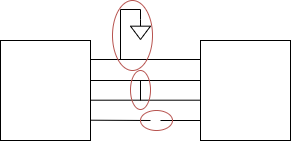
\includegraphics[width=250px]{images/26_JTAG/production_errors.png}
\end{figure}

\subsection{Struttura interna}
Su ogni pin di interesse nel chip inseriamo una piccola rete logica che normalmente conduce e basta:
\begin{figure}[H]
    \centering
    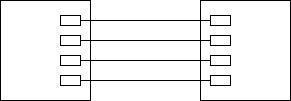
\includegraphics[width=200px]{images/26_JTAG/JTAG_internal.png}
\end{figure}
quando siamo in fase di test tuttavia si può dire a queste reti di porre un valore logico specifico oppure campionare il valore in ingresso.

Questi circuiti sono tutti connessi tra di loro in cascata e vi si comunica in maniera seriale, ci bastano due pin, uno di ingresso alla chain ed uno in uscita dalla chain.
Più chip JTAG possono essere collegati in cascata l' uno con l' altro, questa configurazione è detta \emph{daisy chain}.
Ogni chip ha inoltre un TAP controller (Test Access Port) e più controllori possono essere collegati in parallelo:
\begin{figure}[H]
    \centering
    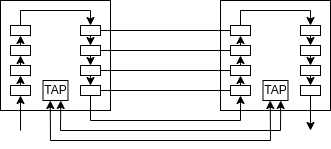
\includegraphics[width=250px]{images/26_JTAG/multiple_JTAG_chips.png}
\end{figure}

\subsection{Collegamenti}
Abbiamo detto che ci servono quindi due pin per la daisy chain e due per il TAP:
\begin{itemize}
    \item TDI: test data in
    \item TDO: test data out
    \item TCK: test clock (al TAP)
    \item TMS: test master (al TAP)
\end{itemize}
l'insieme delle reti nella catena è chiamato \emph{boundary scan chain}.

Ogni chip oltre alla propria daisy chain ha anche alcuni registri utili:
\begin{figure}[H]
    \centering
    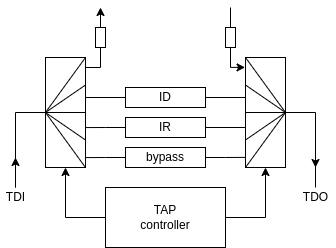
\includegraphics[width=250px]{images/26_JTAG/tap_controller.png}
\end{figure}
\begin{itemize}
    \item ID: registro immutabile che contiene l' id numerico del tipo di chip, è usato per l' identificazione da parte dei debugger e programmatori JTAG
    
    \item bypass: registro ad un bit che obbliga il chip a non fare niente se non propagare i bit in ingresso
    
    \item IR: è l' instruction register
\end{itemize}

\subsection{Funzionamento}
Comunicando con il TAP controller possiamo dire quale registro collegare al multiplexer, successivamente tramite il clock e TDI/TDO possiamo inserire dei bit nella daisy chain, per ogni bit che inseriamo otteniamo un bit in uscita.
Così facendo possiamo ad esempio configurare la connessione con ID ed inserendo bit da un lato leggere i bit dell' ID dall' altro.

Per essere sicuri di star leggendo il valore corretto inviamo un identificativo a 32 bit che non è associato a nessun chip, quando ce lo ritroviamo in uscita allora siamo sicuri di aver finito il giro completamente.

\subsubsection{Istruzioni}
Ogni chip deve implementare almeno 4 istruzioni obbligatorie per essere definito JTAG, inoltre deve averne altre 4 pubbliche e descritte nel datasheet.
Ci possono ovviamente essere tante altre istruzioni private utilizzate dal produttore per effettuare i propri test.

\subsubsection{Lettura}
Prima di poter leggere effettivamente i valori dobbiamo scoprire quanto è lunga la daisy chain, per fare ciò la riempiamo di zeri e contare i bit che servono per riottenere questa lunga sequenza di zeri.
Successivamente dialogando con il TAP impostiamo l' istruzione e poi estraiamo il risultato dopo l' esecuzione.

\subsection{Interno dei moduli}
Ogni elemento della daisy chain è così composto:
\begin{figure}[H]
    \centering
    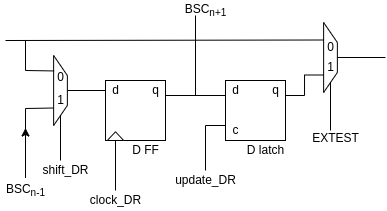
\includegraphics[width=250px]{images/26_JTAG/daisy_chain_element.png}
\end{figure}
i pin shift\_DR, clock\_DR, update\_DR e EXTEST sono tutti in comune e sono pilotati dal TAP.

Attivando shift\_DR attivo il D-flip-flop ed il D-latch in cascata e costruisco un lungo shift register con tutte le altre unità della SBC e con il clock dettato da clock\_DR.
Una volta caricato il valore che voglio posso abilitare update\_DR per ricopiare i valori nel D-latch.
Per portare in uscita al pin il valore scelto devo attivare EXTEST.

Per spiare il valore invece imposto shift\_DR a zero in modo da campionare nel d-flip-flop il valore sul pin e poi faccio scorrere i valori usando shift\_DR.

NB: si noti che questa circuiteria va bene per i pin in uscita, per i pin in ingresso serve altra circuiteria che non vedremo.

\subsection{Utilizzi}
Ad oggi il JTAG oltre ad essere utilizzato per i test in fabbrica è ampiamente utilizzato per il debug e per la programmazione della ROM interna dei chip.
Un software famoso per interfacciarsi con periferiche JTAG è open-OCD.








